%%
%% This is file `sample-authordraft.tex',
%% generated with the docstrip utility.
%%
%% The original source files were:
%%
%% samples.dtx  (with options: `authordraft')
%% 
%% IMPORTANT NOTICE:
%% 
%% For the copyright see the source file.
%% 
%% Any modified versions of this file must be renamed
%% with new filenames distinct from sample-authordraft.tex.
%% 
%% For distribution of the original source see the terms
%% for copying and modification in the file samples.dtx.
%% 
%% This generated file may be distributed as long as the
%% original source files, as listed above, are part of the
%% same distribution. (The sources need not necessarily be
%% in the same archive or directory.)
%%
%% The first command in your LaTeX source must be the \documentclass command.
\documentclass[sigconf,authordraft]{acmart}
% NOTE that a single column version is required for submission and peer review. This can be done by changing the \doucmentclass[...]{acmart} in this template to 
% \documentclass[manuscript,screen]{acmart}

%%
%% \BibTeX command to typeset BibTeX logo in the docs
\AtBeginDocument{%
  \providecommand\BibTeX{{%
    \normalfont B\kern-0.5em{\scshape i\kern-0.25em b}\kern-0.8em\TeX}}}

%% Rights management information.  This information is sent to you
%% when you complete the rights form.  These commands have SAMPLE
%% values in them; it is your responsibility as an author to replace
%% the commands and values with those provided to you when you
%% complete the rights form.
\setcopyright{acmcopyright}
\copyrightyear{2018}
\acmYear{2018}
\acmDOI{10.1145/1122445.1122456}

%% These commands are for a PROCEEDINGS abstract or paper.
\acmConference[Woodstock '18]{Woodstock '18: ACM Symposium on Neural
  Gaze Detection}{June 03--05, 2018}{Woodstock, NY}
\acmBooktitle{Woodstock '18: ACM Symposium on Neural Gaze Detection,
  June 03--05, 2018, Woodstock, NY}
\acmPrice{15.00}
\acmISBN{978-1-4503-XXXX-X/18/06}


%%
%% Submission ID.
%% Use this when submitting an article to a sponsored event. You'll
%% receive a unique submission ID from the organizers
%% of the event, and this ID should be used as the parameter to this command.
%%\acmSubmissionID{123-A56-BU3}

%%
%% The majority of ACM publications use numbered citations and
%% references.  The command \citestyle{authoryear} switches to the
%% "author year" style.
%%
%% If you are preparing content for an event
%% sponsored by ACM SIGGRAPH, you must use the "author year" style of
%% citations and references.
%% Uncommenting
%% the next command will enable that style.
%%\citestyle{acmauthoryear}

\usepackage{caption}
\usepackage{subcaption}

%%
%% end of the preamble, start of the body of the document source.
\begin{document}

%%
%% The "title" command has an optional parameter,
%% allowing the author to define a "short title" to be used in page headers.
\title{The Name of the Title is Hope}

%%
%% The "author" command and its associated commands are used to define
%% the authors and their affiliations.
%% Of note is the shared affiliation of the first two authors, and the
%% "authornote" and "authornotemark" commands
%% used to denote shared contribution to the research.
\author{Ben Trovato}
\authornote{Both authors contributed equally to this research.}
\email{trovato@corporation.com}
\orcid{1234-5678-9012}
\author{G.K.M. Tobin}
\authornotemark[1]
\email{webmaster@marysville-ohio.com}
\affiliation{%
  \institution{Institute for Clarity in Documentation}
  \streetaddress{P.O. Box 1212}
  \city{Dublin}
  \state{Ohio}
  \postcode{43017-6221}
}

\author{Lars Th{\o}rv{\"a}ld}
\affiliation{%
  \institution{The Th{\o}rv{\"a}ld Group}
  \streetaddress{1 Th{\o}rv{\"a}ld Circle}
  \city{Hekla}
  \country{Iceland}}
\email{larst@affiliation.org}

\author{Valerie B\'eranger}
\affiliation{%
  \institution{Inria Paris-Rocquencourt}
  \city{Rocquencourt}
  \country{France}
}

\author{Aparna Patel}
\affiliation{%
 \institution{Rajiv Gandhi University}
 \streetaddress{Rono-Hills}
 \city{Doimukh}
 \state{Arunachal Pradesh}
 \country{India}}

\author{Huifen Chan}
\affiliation{%
  \institution{Tsinghua University}
  \streetaddress{30 Shuangqing Rd}
  \city{Haidian Qu}
  \state{Beijing Shi}
  \country{China}}

\author{Charles Palmer}
\affiliation{%
  \institution{Palmer Research Laboratories}
  \streetaddress{8600 Datapoint Drive}
  \city{San Antonio}
  \state{Texas}
  \postcode{78229}}
\email{cpalmer@prl.com}

\author{John Smith}
\affiliation{\institution{The Th{\o}rv{\"a}ld Group}}
\email{jsmith@affiliation.org}

\author{Julius P. Kumquat}
\affiliation{\institution{The Kumquat Consortium}}
\email{jpkumquat@consortium.net}

%%
%% By default, the full list of authors will be used in the page
%% headers. Often, this list is too long, and will overlap
%% other information printed in the page headers. This command allows
%% the author to define a more concise list
%% of authors' names for this purpose.
\renewcommand{\shortauthors}{Trovato and Tobin, et al.}

%%
%% The abstract is a short summary of the work to be presented in the
%% article.
\begin{abstract}

\end{abstract}

%%
%% The code below is generated by the tool at http://dl.acm.org/ccs.cfm.
%% Please copy and paste the code instead of the example below.
%%
\begin{CCSXML}
<ccs2012>
 <concept>
  <concept_id>10010520.10010553.10010562</concept_id>
  <concept_desc>Computer systems organization~Embedded systems</concept_desc>
  <concept_significance>500</concept_significance>
 </concept>
 <concept>
  <concept_id>10010520.10010575.10010755</concept_id>
  <concept_desc>Computer systems organization~Redundancy</concept_desc>
  <concept_significance>300</concept_significance>
 </concept>
 <concept>
  <concept_id>10010520.10010553.10010554</concept_id>
  <concept_desc>Computer systems organization~Robotics</concept_desc>
  <concept_significance>100</concept_significance>
 </concept>
 <concept>
  <concept_id>10003033.10003083.10003095</concept_id>
  <concept_desc>Networks~Network reliability</concept_desc>
  <concept_significance>100</concept_significance>
 </concept>
</ccs2012>
\end{CCSXML}

\ccsdesc[500]{Computer systems organization~Embedded systems}
\ccsdesc[300]{Computer systems organization~Redundancy}
\ccsdesc{Computer systems organization~Robotics}
\ccsdesc[100]{Networks~Network reliability}

%%
%% Keywords. The author(s) should pick words that accurately describe
%% the work being presented. Separate the keywords with commas.
\keywords{datasets, neural networks, gaze detection, text tagging}

%% A "teaser" image appears between the author and affiliation
%% information and the body of the document, and typically spans the
%% page.

%%
%% This command processes the author and affiliation and title
%% information and builds the first part of the formatted document.
\maketitle

\section{Introduction}


\section{Background}

\subsection{College Application Process}
The automated college admission system is providing the SSC (Secondary School Certifacte) passed students a user friendly platform to apply for their desired colleges. The current automated system is serving from the academic year 2007-18 ?? and almost 1.3 millions of students submit their college choices under this application system. 
Proir to the application process, the applying student need to make the payment according to the general guideline published by Bangladesh Inter-education Board Coordination Subcommittee. For example, the gudeline of the year 2020 directs that the applicants need to pay BDT150 through one of the registered Payment Service Providers (PSP); i) Nagad \cite{nagad}, ii) Sonali bank \cite{sonalibank}, iii) Teletalk \cite{teletalk}, iv) bKash \cite{bkash}, v) Rocket \cite{rocket}. 
As soon as the payment is confirmed, an applicant can start his/her application process by clicking the Apply Now button on the landing page of the web application of XI Admission System \cite{xiaddmissionlandingpage} (shown in Figure \ref{fig:landing}). The button redirects the applicant to one of its existing application servers. This allocation is done using a DNS based load balancer that performs a modulus arithmatic on the timestamp of clicking the Apply Now button. All the services to the applicant is served from this specific application server. The applicant then need to get into the main application process by inputing his/her SSC Roll No, Board, Passong Year and Registration No as shown in Figure \ref{fig:login}. After logging into into the system, the applying student need to verify the contact no he have submitted during the payment procedure (Figure \ref{fig:contact_check}). A successfull verification brings the applicant to the college choice page as shown in the Figure \ref{fig:choice}. 
Each college of admission system is identified by an id named \textit{EIIN}. Each college can have:
\begin{itemize}
	\item multiple shifts such as Morning, Day, etc. which can be idenfied by \textit{Shift ID} \item two possible versions such as English, Bangla which can be identified by \textit{Version ID}
	\item multiple groups such as Science, Humanities, Business Studies, etc. which can be identified by \textit{Group ID}
\end{itemize}
Now each college choice is a unique tuple of (EIIN, Shift ID, Version ID, Group ID) and can be termed as an ESVG choice. An applicant can add an arbitrary number of ESVG choice while keeping the count of unique EIIN within a range of minimum of five and a maximum of ten. 


\begin{figure*}[t]
	\centering
	\begin{subfigure}{.48\linewidth}
		
\includegraphics[width = \linewidth]{landing_page}
		\caption{Application Landing Page}
		\label{fig:landing}
	\end{subfigure}
	\begin{subfigure}{.48\linewidth}
		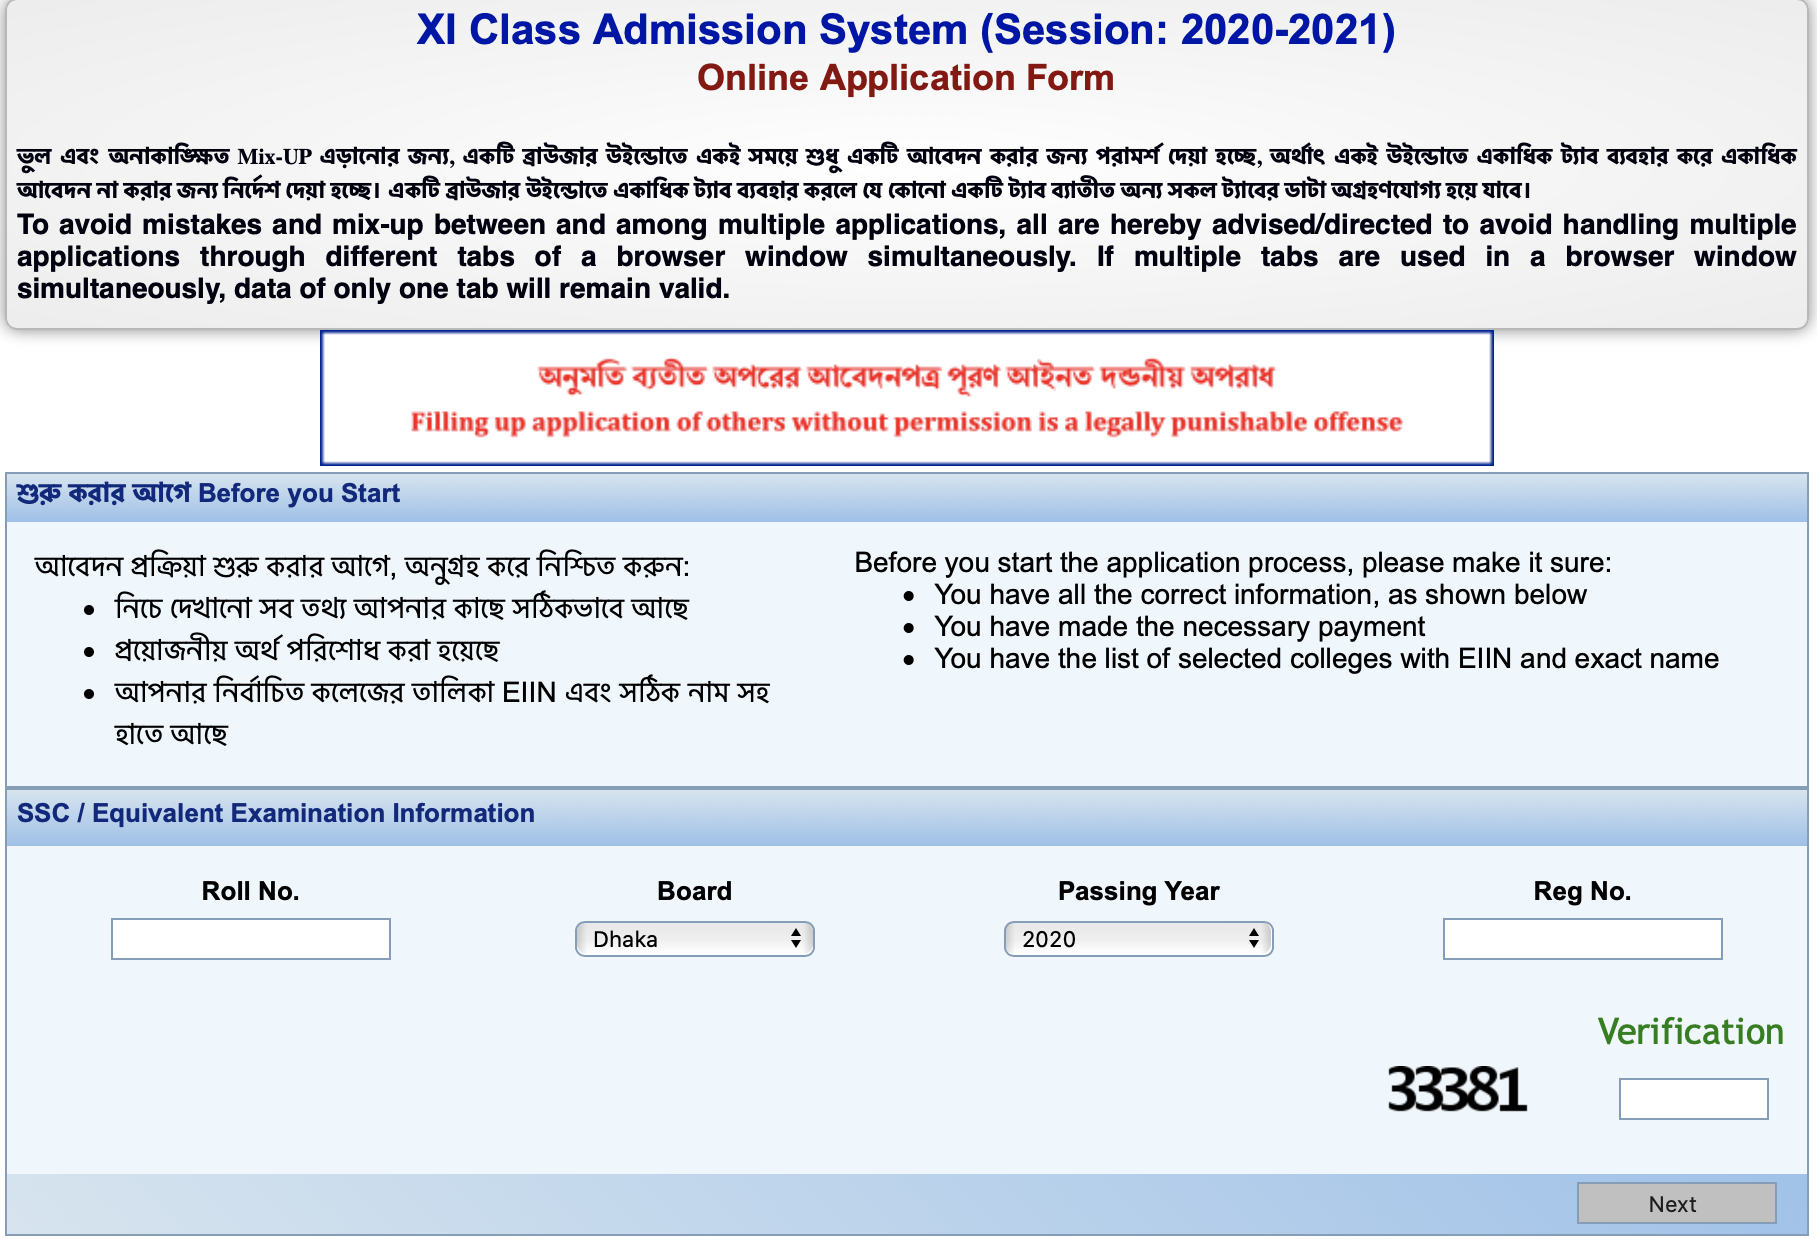
\includegraphics[width = \linewidth]{log_in_page}
		\caption{Student Log In Page}
		\label{fig:login}
	\end{subfigure}
	\begin{subfigure}{.48\linewidth}
		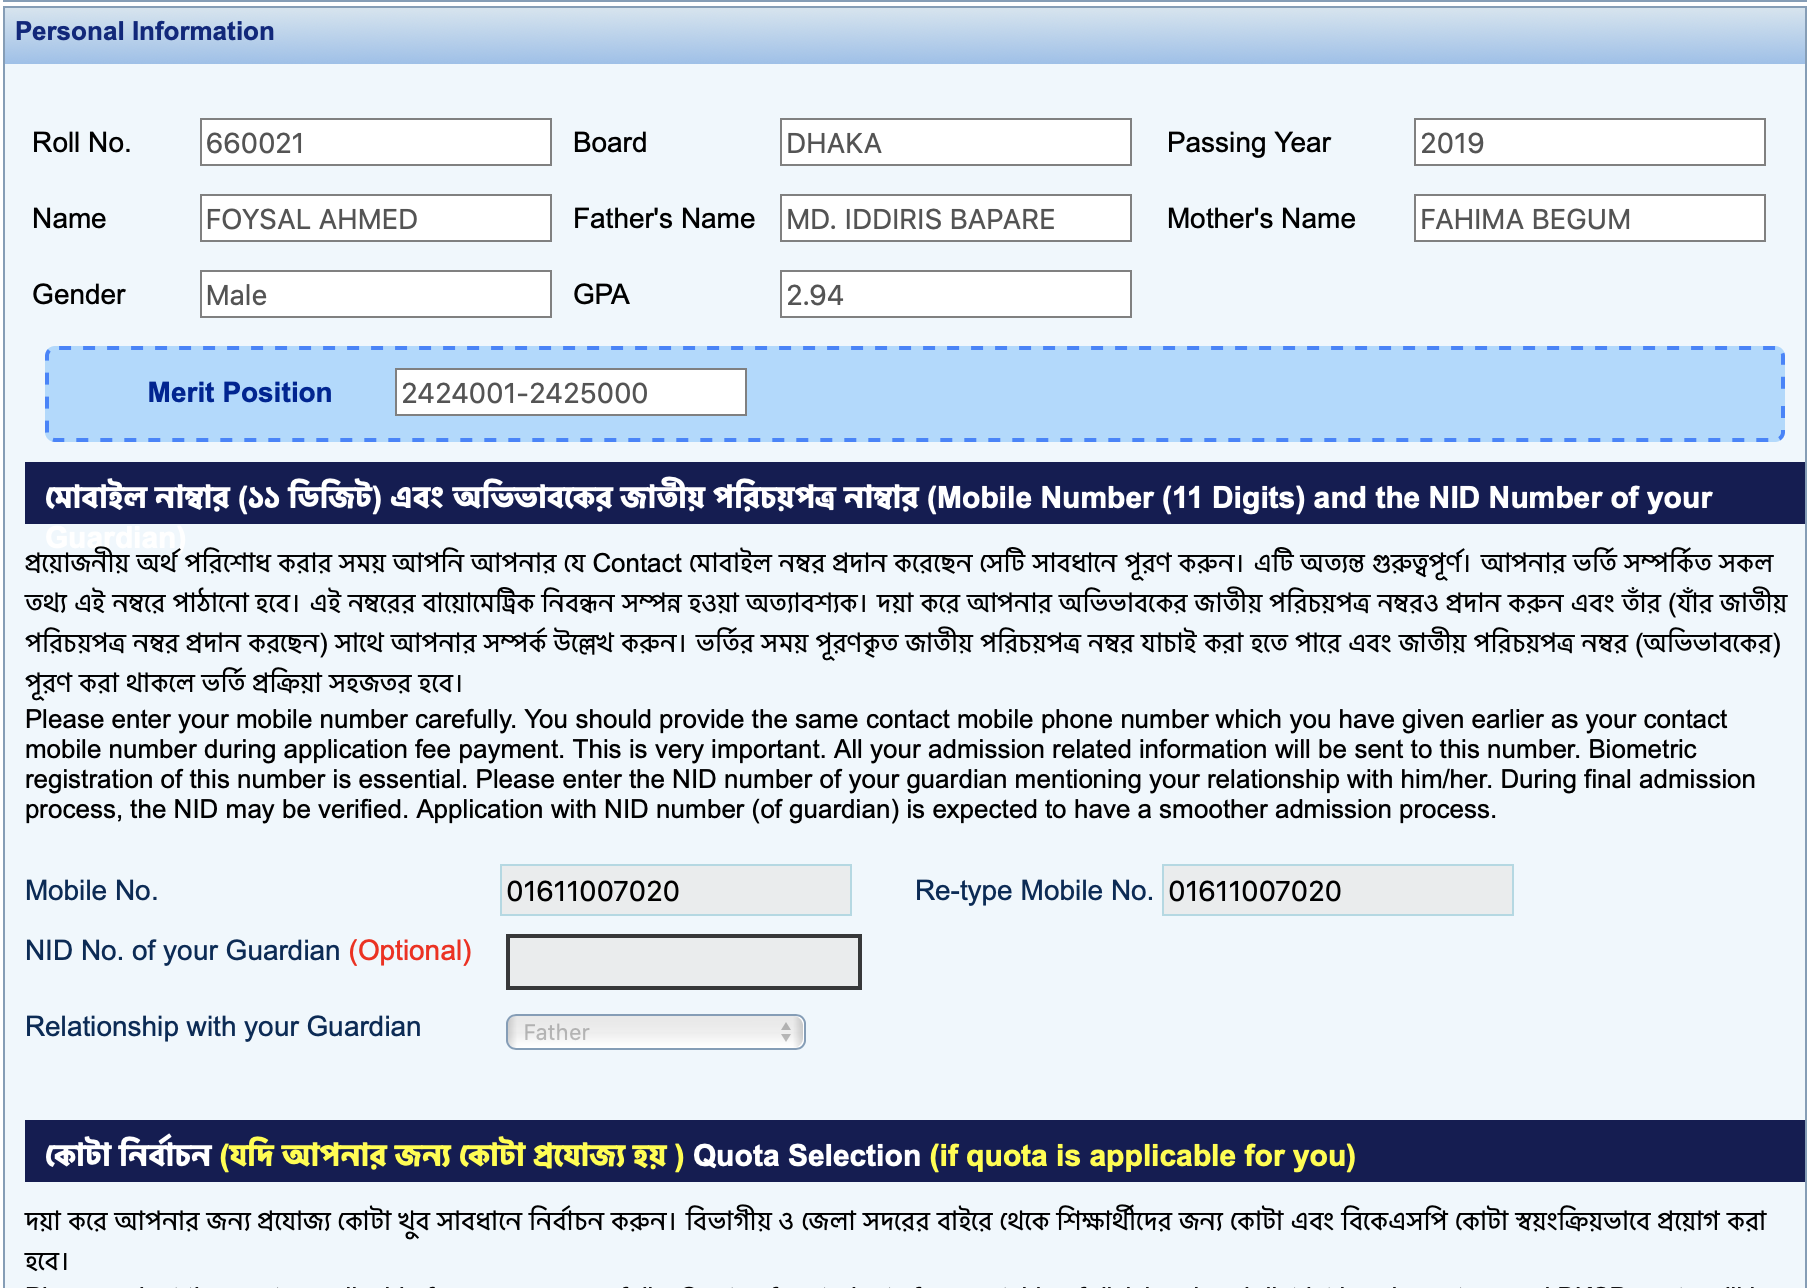
\includegraphics[width = \linewidth]{contact_check}
		\caption{Contact Number Validation Page}
		\label{fig:contact_check}
	\end{subfigure}
	\begin{subfigure}{.48\linewidth}
		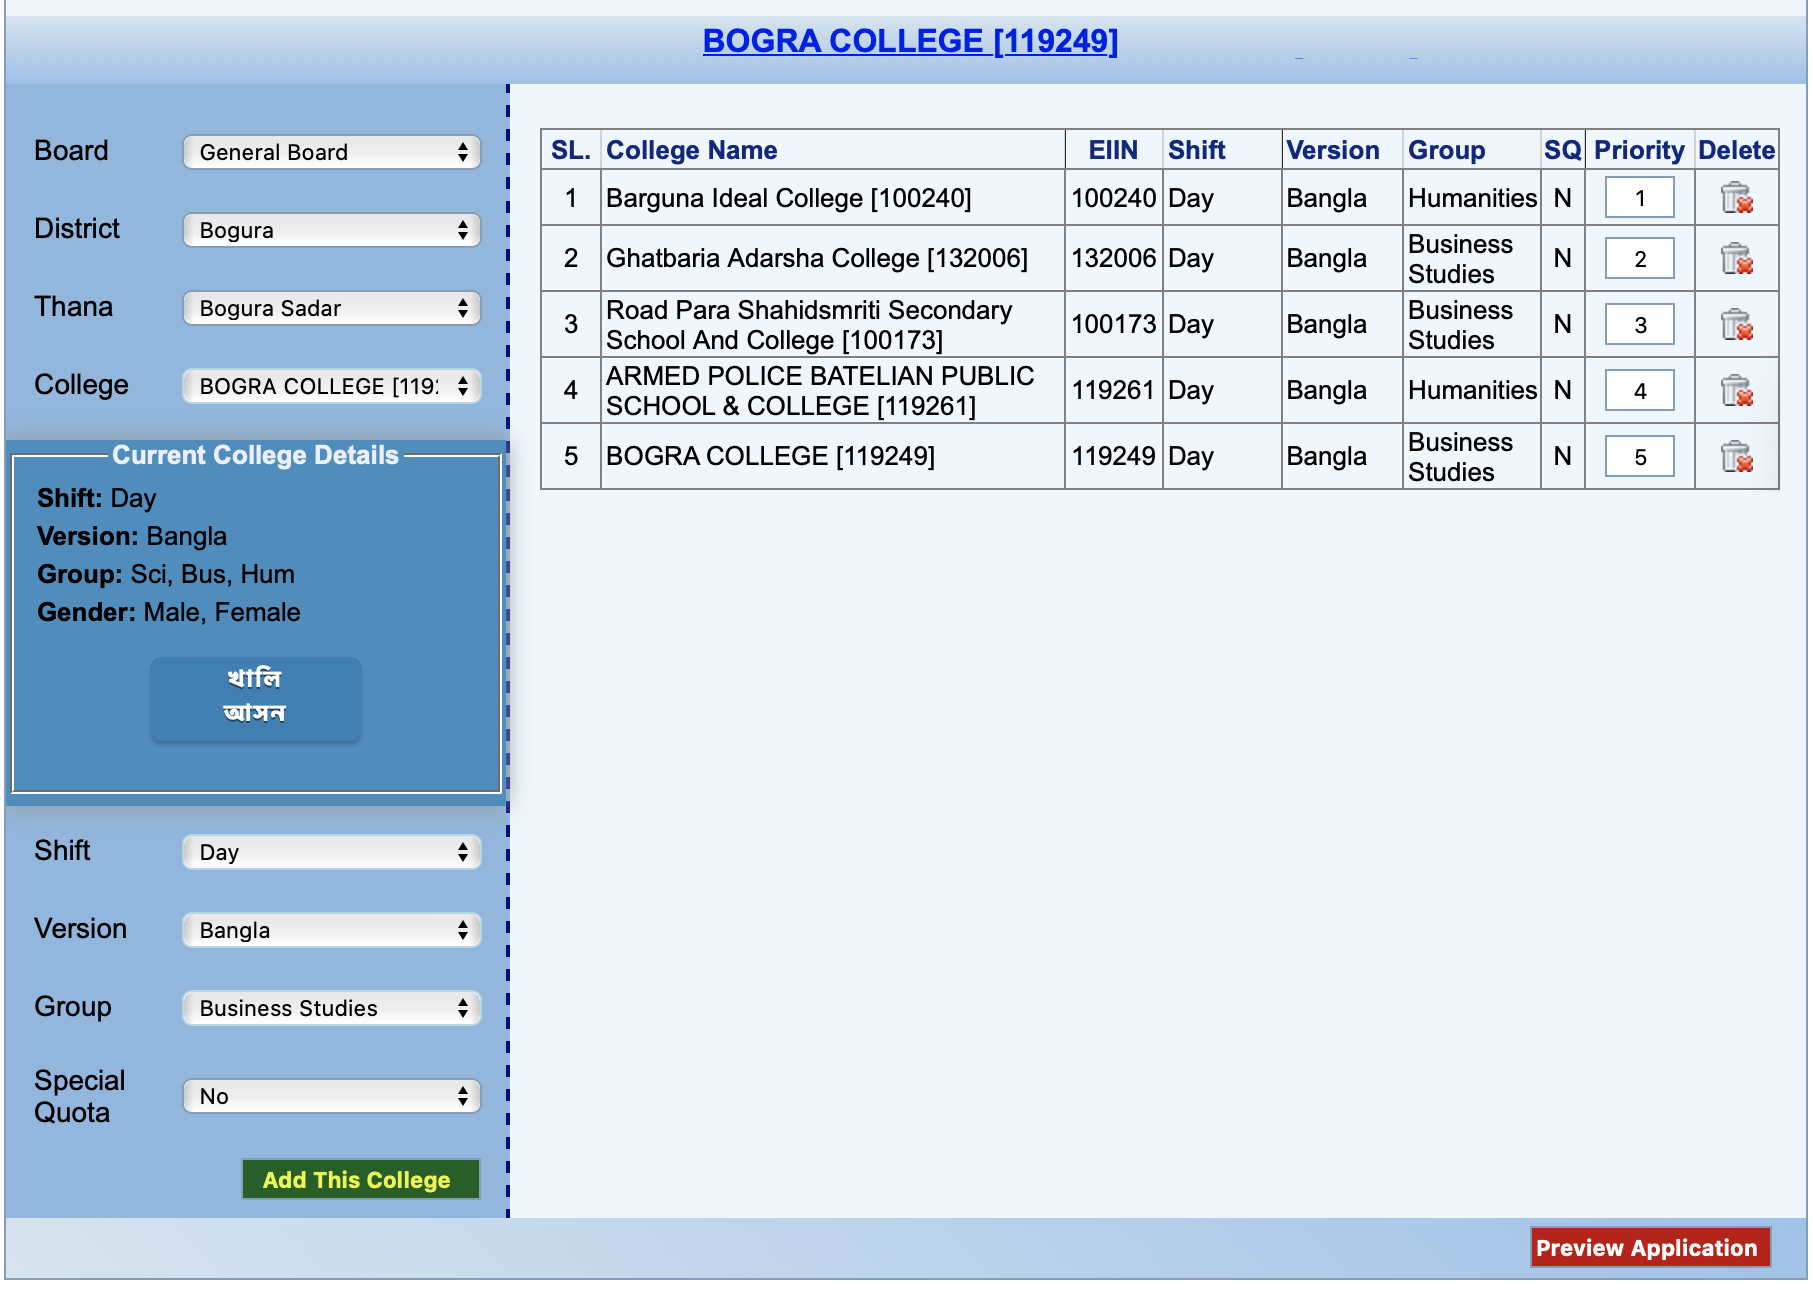
\includegraphics[width = \linewidth]{choice_page}
		\caption{Application College Choice Page}
		\label{fig:choice}
	\end{subfigure}
\caption{Screenshots of Web Application of XI Class Admission System}
\label{fig:screenshots}
\end{figure*}   

\subsection{Load Testing}

\subsection{Load Testing Tools}

\section{Environment Setup}
We conduct our load testing on three different environment; i) on the test bed, ii) on the production environment in projected load scneario, and iii) on the live application website in real scenario. The test environment is initially set up on a local server at the IICT. Testing on the test bed allows the authors to prepare a proper test plan and a benchmark to evaluate the performance of the final environment. 
%Each of the environments is comprised of one or multiple 

\subsection{Server Configuration}
\subsubsection{Test Environment}
The test environment is comprised with a single application server and a single database server running on Oralce 12c ? [?cite?]. The configuration of the test bed is as follows.
\begin{itemize}
	\item Application server has 16 GB of RAM, 1 CPU, and 1 tomcat server running with 8 GB allocated memory.
	\item Database (DB) server has 24 GB of RAM and 1 CPU.
	\item Maximum allowed connections on the oracle DBMS
	\begin{itemize}
		\item Session 252
		\item Process 150
		\item Open Cursor 300
	\end{itemize}
	\item Maximum 30 connections in the connection pool from each tomcat to database.
\end{itemize}

\subsubsection{Production Environment}
As the time of main application reaches nearer, the college admission application system is deployed on a production environment with higher configuration setup. 
The production environment is built on the virtual machines hosted by the renowned cloud service provider named ``Brilliant Cloud". This production environment is comprised of six application server and a single Oracle database server. 
All the tests from the test server are replicated on the production server and it is expected to get a significantly better performance from the test server. 
The 
The configuration of the production environment for College Admission 2020 is as follows.
\begin{itemize}
	\item Each of the six Application servers has 32 GB of RAM, 8 core processor, and 100 GB Storage. 
	\item Single Payment server has 32 GB of RAM, 8 core processor, and 100 GB of Storage.
%	- Static website server (Do not know the configuration yet)
	\item Single database server has 128 GB of RAM, 16 core processor,  and 280 GB SSD Storage.
	\item Maximum allowed connections on the oracle DBMS
	\begin{itemize}
		\item Session $\sim$ 1.5 $\times$ Process
		\item Process 2500
		\item Open Cursor 4000
		\item shared server 1,
		\item hared pool = 0
	\end{itemize}
	\item Provision of dedicated server which means 1 process is 1 dedicated connection. 
\end{itemize}

\subsection{Load Balancing on Production Environment}

As we already have mentioned that the final environent is comosed of six appliation servers which are used for load balancing. The college admission applicaton system uses DNS based load balancing technique. 
DNS load balancing is a software-defined approach to load balancing where client requests to a domain within the Domain Name System (DNS) are distributed across different server machines. The DNS system sends a different version of the list of IP addresses each time it responds to a new client request using the round-robin method, therefore distributing the DNS requests evenly to different servers to handle the overall load. This in turn provides DNS load balancing failover protection through automatic removal of non-responsive servers. 
Each time a client is trying to hit the application page, the timestamp is recorded, and based on the modulus arithmatic on this timestamp, the client is directed to a specific server among the six to handle his process of application. 

Figure \ref{fig:architecture} shows the system architecture of the college admission application system. Each pf six application server are tagged with xiapp2--xiapp7. 

\begin{figure}[h]
	\centering
	\fbox{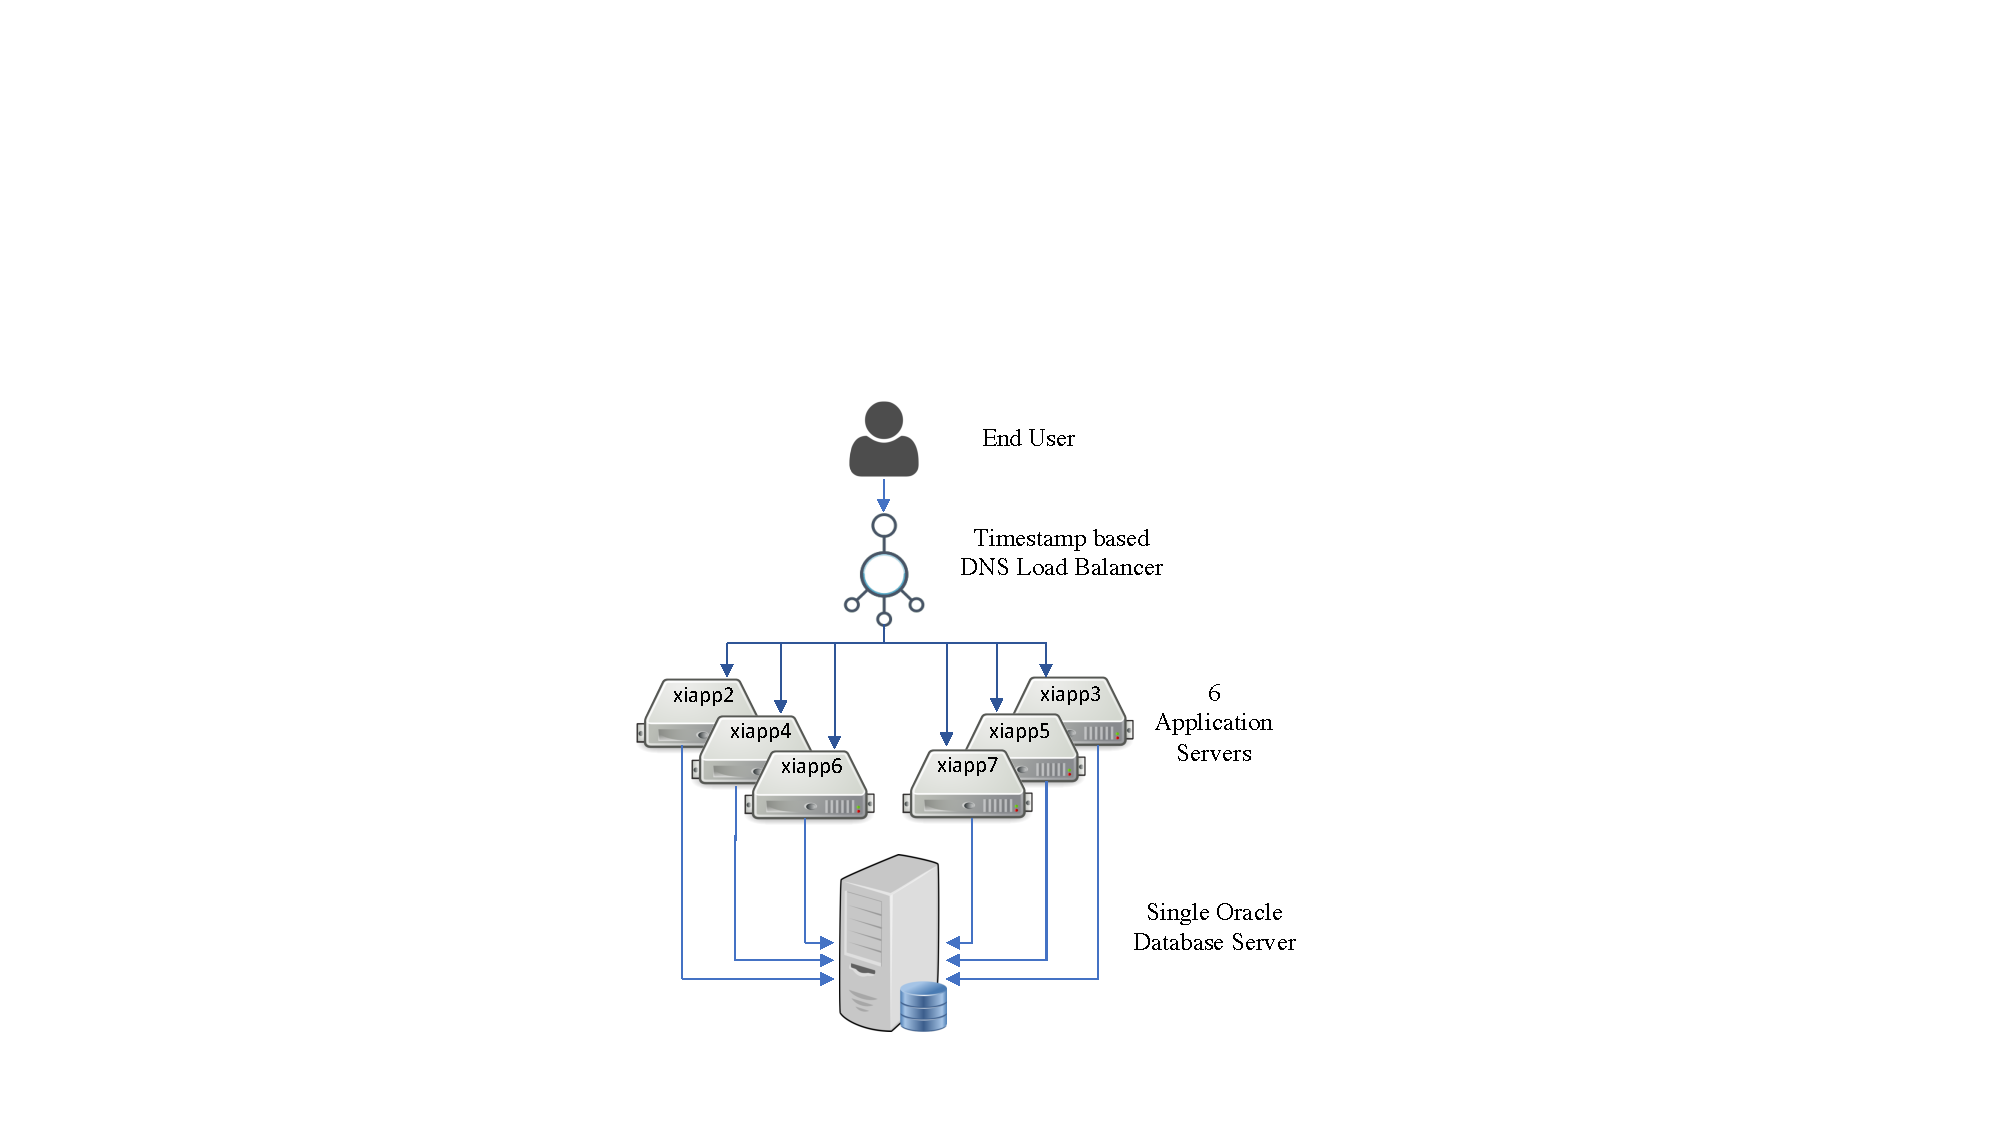
\includegraphics[width=\linewidth]{architecture}}
	\caption{Artchitecture of the Final Production Environemnt}
	\Description{Artchitecture of the Final Production Environemnt}
	\label{fig:architecture}
\end{figure}


\section{Test Plan}
We prepare a suitable test plan for this year's application system based on the historical data of last years. The following historical data is extracted from the college admission application process of 2019.
\begin{itemize}
	\item Maximum hourly load was $\sim 18684$ applications, which happened at mid-day of day-1.
	\item 38 applications per second is a burst rate that happens in around mid-day.
	\item Applicant count was 1373387.
	\item No of SMS applications: 349986, No of WEB applications: 5741143. 
	\item ESVG count 6091129. Therefore, average ESVG by a student was $\sim 4.5$.
	\item Maximum ESVG choices done by a student was $\sim 28$.
\end{itemize}
Based on the statistics from the previous year, a load projection plan is prepared as follows.
\begin{itemize}
	\item We plan to load the system with a maximum hourly rate of 25000 application.
	\item The server performance should be examined by generating a varying rate of load between 5000 applications/hour and the maximum rate.
	\item Since there are database read and write operation involved in the application process, the impact of database size on the application response times is needed to be examined.
	\item We plan to observe that if a burst rate of at least 50 is generated under the projected load scenario.
	\item The performance shold be tested by generating a varied number of concurrent connections. The target is to exhaust the system with high number of simutaneous connection and observe that if it can sustain with acceptable performance.
\end{itemize}
We should keep in mind that the test server may not be able to meet all our desired performance. However, we are intended to have a clear visualization on how well the production server is going to perform in real load scenario.

\section{Evaluation Metrics}
We use the following metrics to evaluate the response time of each of the HTTP requests as well as the full application procedure. 
\begin{itemize}
	\item Average
	\item Median
	\item $90^{th}$ Percentile
	\item $95^{th}$ Percentile
	\item $99^{th}$ Percentile
\end{itemize}

In addition, we also use the percentage of error as an evaluation metric to assess how successfully the requests are served by the application and database server. 




\section{Experimental Outcome}
\subsection{Varied Load Projection}
As we have discussed earlier, we project a load of application processes which we vary from 5000 applications/hour to a maximum of 25000 applications/hour rate. This test is carried out on both the test bed and the prduction environment. 
Each rate is generated for multiple times and an average is considered. During this test the load was generated from a machine which is connceted to a network different from the network where the application and database server are hosted.  
The main intention of this test is to assess if the application system can provide services in a consistent manner and reach the maximum rate of application without compromising in the performace. Figure \ref{fig:varied_load} demonstrate the variation in response times with the variation in projected load. It can clearly be observed that the preformance of the production environment is more stable with a shorter range of variation. 


\begin{figure*}
	\centering
	\begin{subfigure}{0.5\linewidth}
		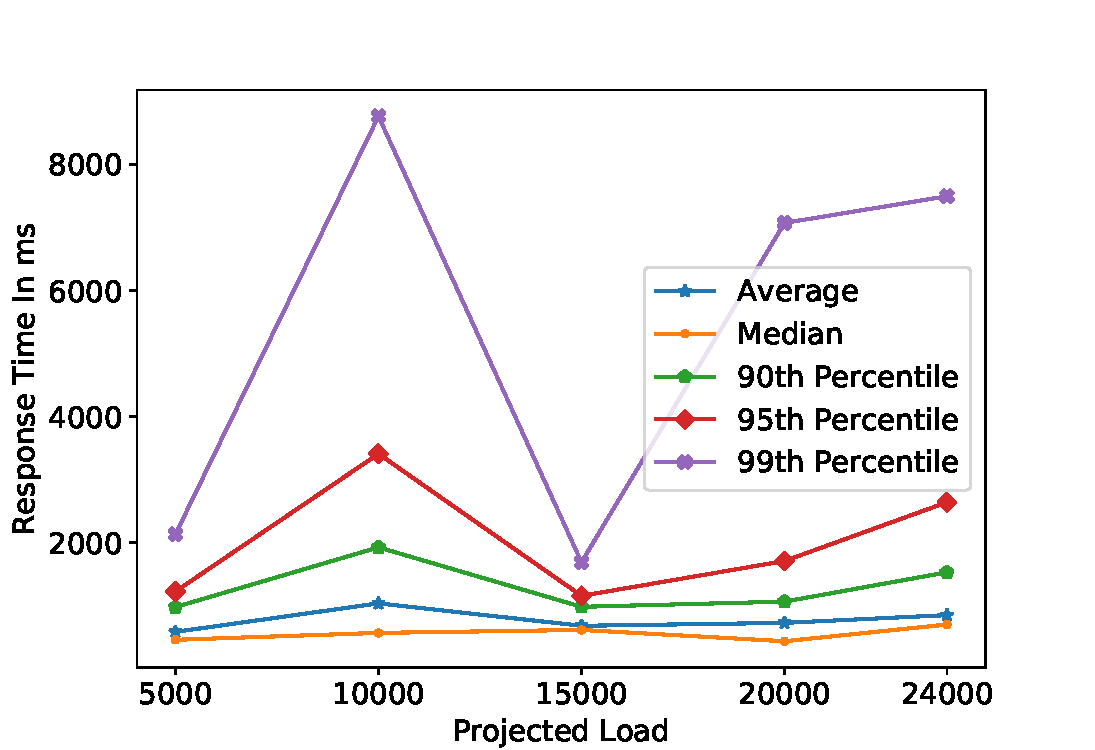
\includegraphics[width=\linewidth]{Test_Bed_Varied_Load}
		\caption{Test Environment}
		\label{fig:varied_load_tes}
	\end{subfigure}
	\begin{subfigure}{0.49\linewidth}
		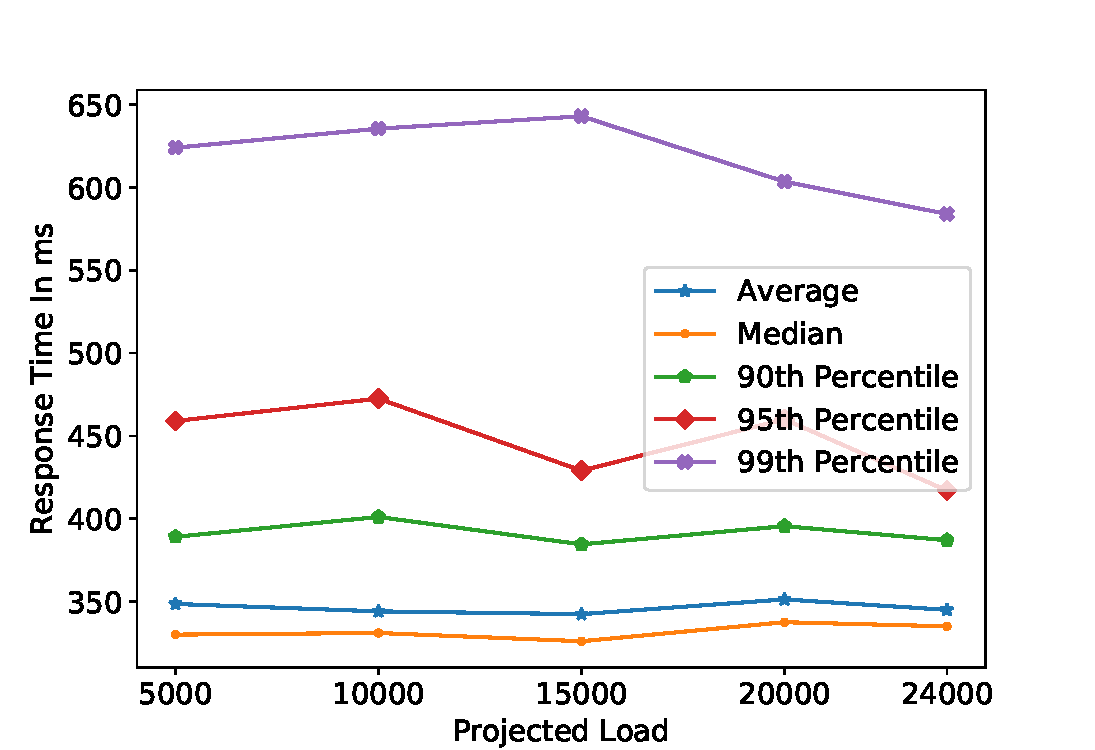
\includegraphics[width=\linewidth]{Production_Varied_Load}
		\caption{Production Environment}
		\label{fig:varied_load_final}
	\end{subfigure}
\caption{Change in Response Times with Varied Load}
\label{fig:varied_load}
\end{figure*}

\subsection{Impact of Database Partitioning}



\subsection{Imapct of Database Size}
Each application process is started with a database query which search the details information of the applicant with the Roll No, Board, Passing Year, and Registration No provided at the log in page of Figure \ref{fig:login}. On the other hand, this process is ended with a database with of the applicant's college choices. Therefore, we intend to observe the impact of database size on the response times of the application processes. To evaluate that, we submit more than 400 thousand full applications each of which submits 10 ESVG choices. 

Note that we perform these experiments at a fixed load of 20,000 applications per hour. The machines which are used to generate load for both test bed and final environment are connected with the same corresponding networks where the application and database servers are running. However, for the final environment, since the network bandwidth provided by ``Billiant Cloud" is very high, the response times are similar for machines outside the system's network.
 
Figure \ref{fig:db impact} shows the impact of database size on the response times based on the previously mentioned metrics. Each graph shows the response times of a full application process for both the test and production environment. 

Graphs are drawn for top two time consuming HTTP requests, ``Application Log In" and ``Application Submission" and the time requirement of a full application process. The response time are considerably flat with respect to the size of the database. However there is a spike for database size of 50,000 which can be an outcome of randomly introduced network latency. 
On the other hand, Figure \ref{fig:db impact final} shows the similar results when the tests are conducted on the final environment. One point is cleat that, for both cases the response times stay considerably flat with the variation of database size. However, for the final server, all the response times are increased by some amount. For example, the median response time of the HTTP request for ``Application Submission" takes $60ms$ in the test environment. In contrary, it is increased to around $140ms$ in the final environment. This is because of the slower database write operation which is caused by a slower SSD storage media of the virtual machines provided by ``Brilliant Cloud". However, since all the response times were consistent and within a tolerable limit of delay, the test results were accepted by the Quality Assurance Team. 

\begin{figure*}
	\centering
	\begin{subfigure}{0.49\linewidth}
		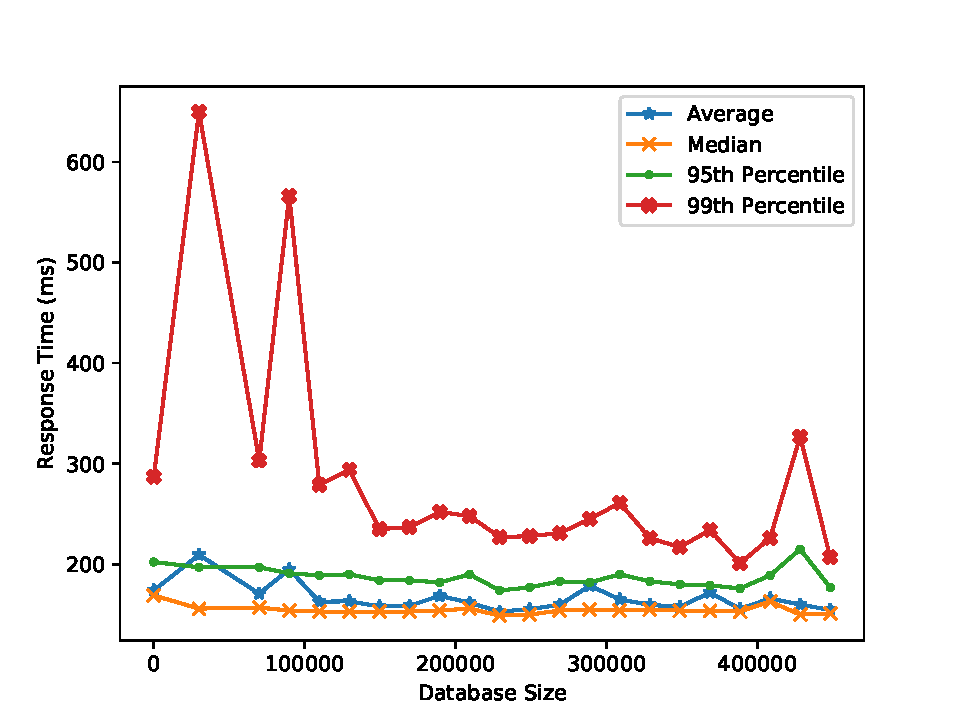
\includegraphics[width=\linewidth]{test_db}
		\caption{Test Environment}
		\label{fig:test_db}
	\end{subfigure}
	\begin{subfigure}{0.49\linewidth}
		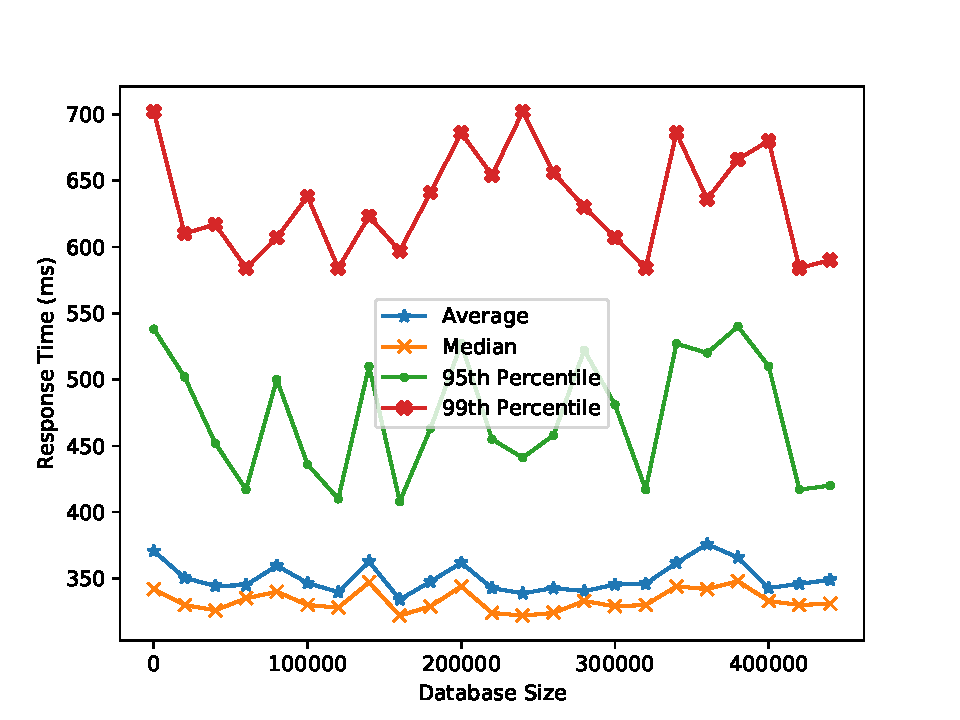
\includegraphics[width=\linewidth]{final_db}
		\caption{Production Environment}
		\label{fig:final_db}
	\end{subfigure}
\caption{Impact of Database Size on Response Times}
\label{fig:db_impact}
\end{figure*}


\subsection{Varied Concurrent Connections}
We vary the number of concurrent connections for both the test environment and the final production environment and record the response times for each of the HTTP requests as well as the full application process. 
%Note that generating concurrent connection more than 3500 was not feasible due to operating system limitation. 
We demonstrate the outcoms graphically in Figure \ref{fig:con_impact}. 

Firstly, Figure \ref{fig:concurrency_1} and Figure \ref{fig:final_concurrency_1} show the results graphically for the test and final environments repectively. The Thana Retrieval, College Retrieval, College SVG Retrieval lines are drawn by averaging within all the existing HTTP requests executing the corresponding retrieval tasks. We can observe that response time of each kind tends to increase with the increased number of concurrent connections. 
On the other hand, except from some spikes in the landing pages, the response times for the main requests stay flat which bears the testimony that the final server is capable for serving smoothly under high concurrent load condition.

Secondly, Figure \ref{error_concurrency} shows the error generated with the increment in concurrency level. We can observe that the error rate stays within very small margin (maximum $1.4\%$ to be specific) for the final environment which is comparatively higher (up to $10\%$) in the test environment.

Finally, Figure \ref{full_package_concurrency} shows response times based on different kind of metrics for full application process with varied concurrency rate. In case of the test conducted on the test environment, we can observe that all the metrics is increasing with the incease in concurrency while for the final environment, the average and median response times are staying sufficiently flat in the curves that provides the verdict that the final environment is very capable of performing consistently under high concurrent connections.   

From the experiment we perform by varying the number of concurrent connection, we can conclude that the application servers in both the test and final environments are successful to serve within a tolerable error margin with a decent performance even with a large number of concurrent connections. We should keep in mind that the test environment consists of a single server machine while the final production environment has six such server machines to serve in parallel. Therefore, it is very expected that the final environment is delivering significantly better performance.


\begin{figure*}
	\centering
	\begin{subfigure}{0.49\linewidth}
		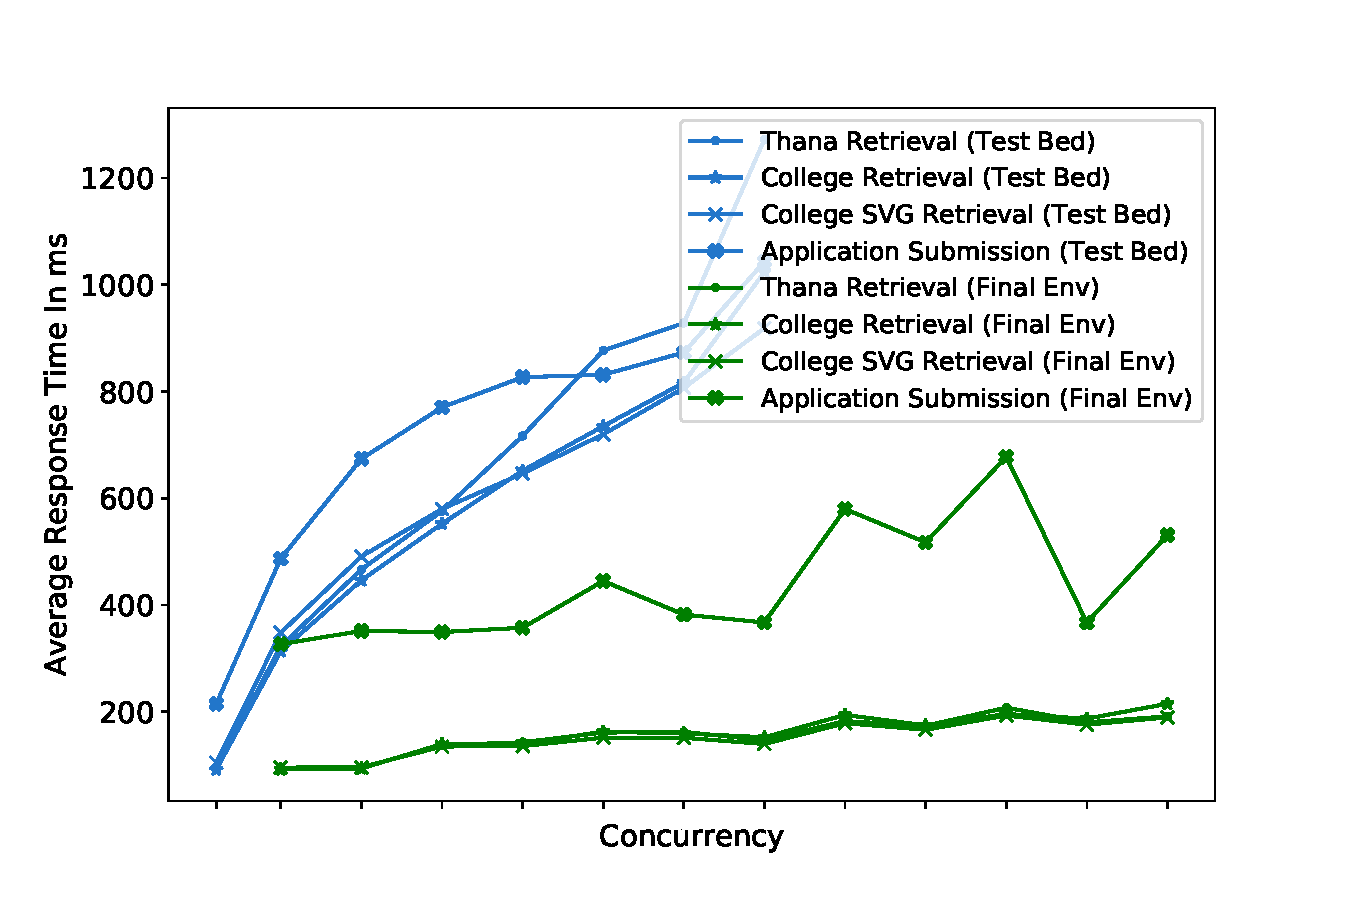
\includegraphics[width=\linewidth]{Average_con}
		\caption{}
		\label{fig:avg_con}
	\end{subfigure}
	\begin{subfigure}{0.49\linewidth}
		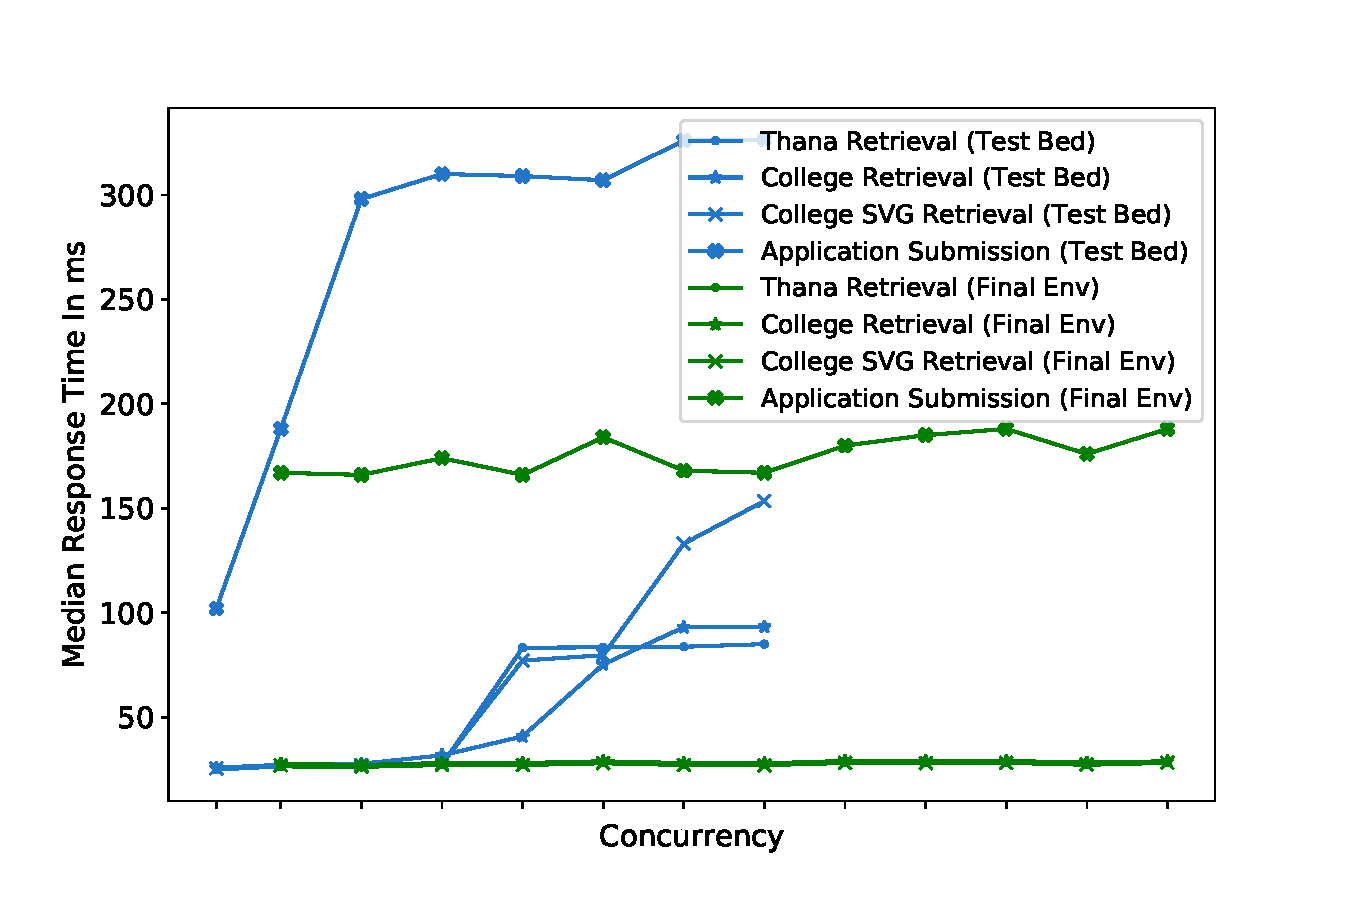
\includegraphics[width=\linewidth]{Median_con}
		\caption{}
		\label{fig:med_con}
	\end{subfigure}
	\begin{subfigure}{0.49\linewidth}
		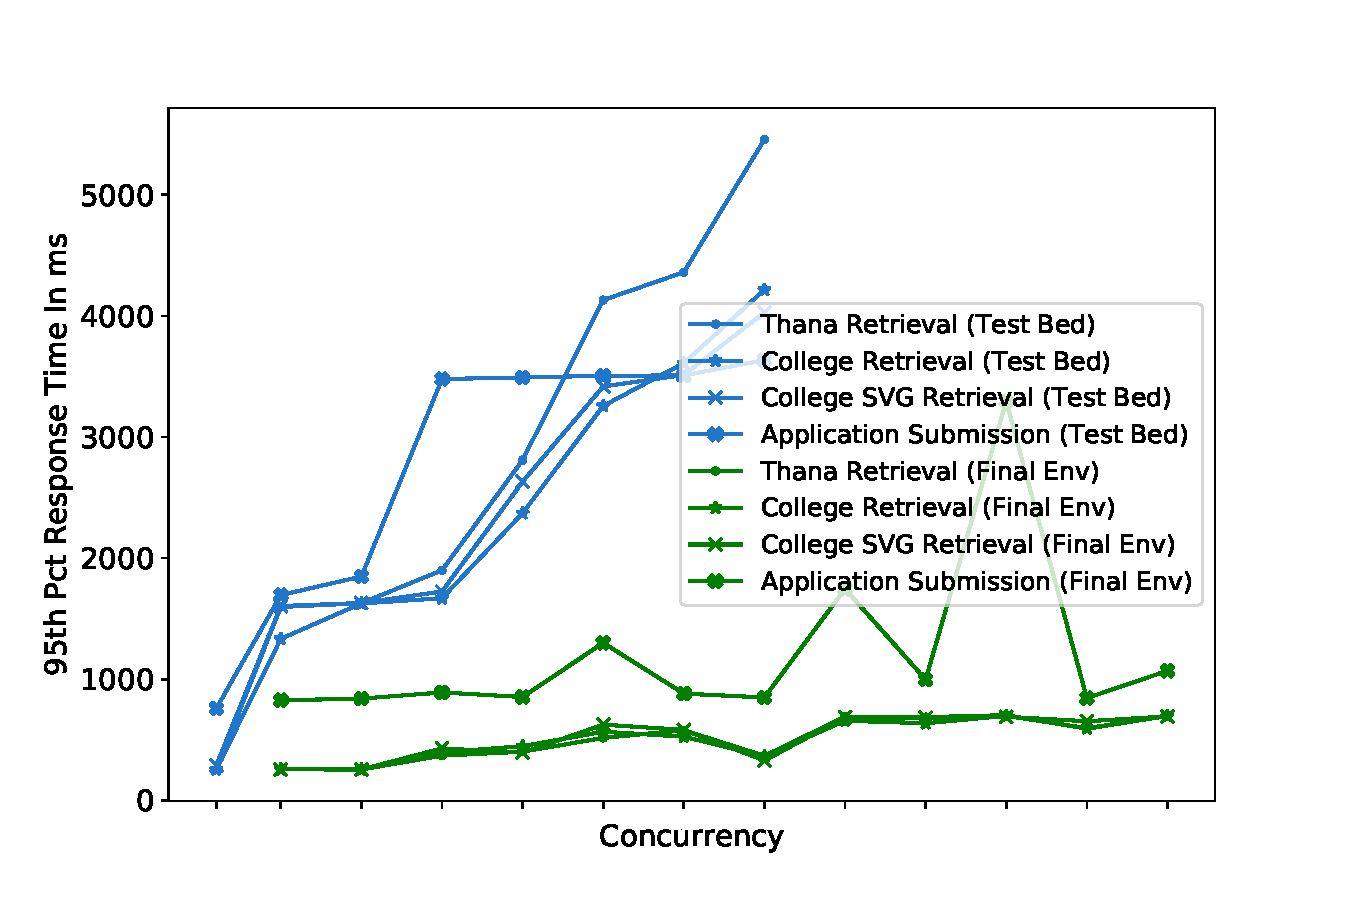
\includegraphics[width=\linewidth]{95th_con}
		\caption{}
		\label{fig:95th_con}
	\end{subfigure}
	\begin{subfigure}{0.49\linewidth}
		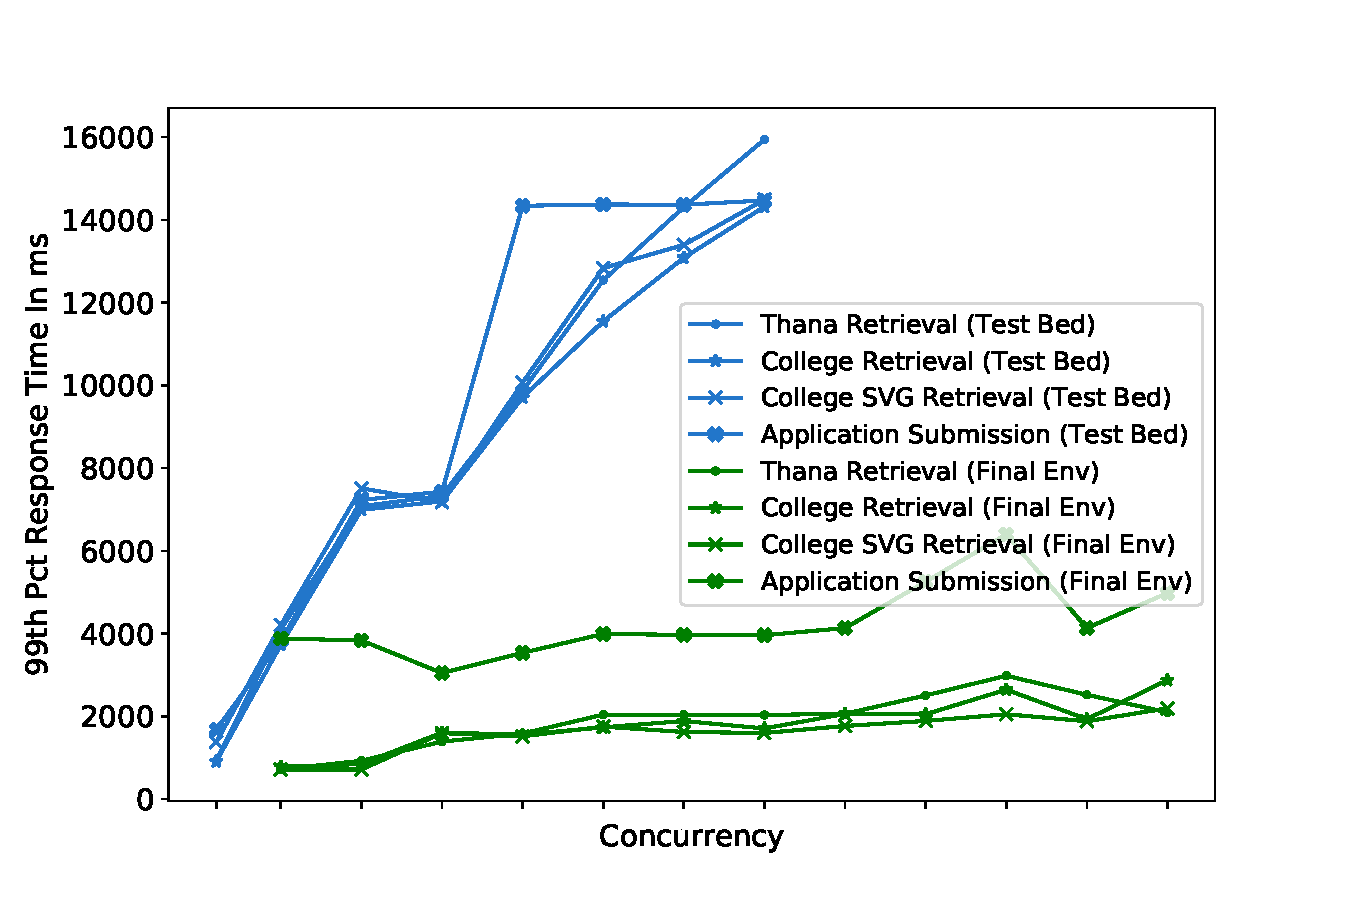
\includegraphics[width=\linewidth]{99th_con}
		\caption{}
		\label{fig:99th_con}
	\end{subfigure}
	\caption{Impact of Varied Concurrent Connections on Response Times}
	\label{fig:con_impact}
\end{figure*}


%%
%% The next two lines define the bibliography style to be used, and
%% the bibliography file.
\bibliographystyle{ACM-Reference-Format}
\bibliography{sample-base}

%%
%% If your work has an appendix, this is the place to put it.


\end{document}
\endinput
%%
%% End of file `sample-authordraft.tex'.
